\chapter{Background and Related Work}
\label{sec:previousworks}
Bla Bla

\begin{quotation}
\textit{CR is a radio that can change its transmitter parameters based on its interaction with the environment in which it operates. This interaction may involve active negotiation or communications with other spectrum users and/or passive sensing and decision making within the radio.}
\end{quotation}

\begin{figure}[!htb]
\begin{center}
	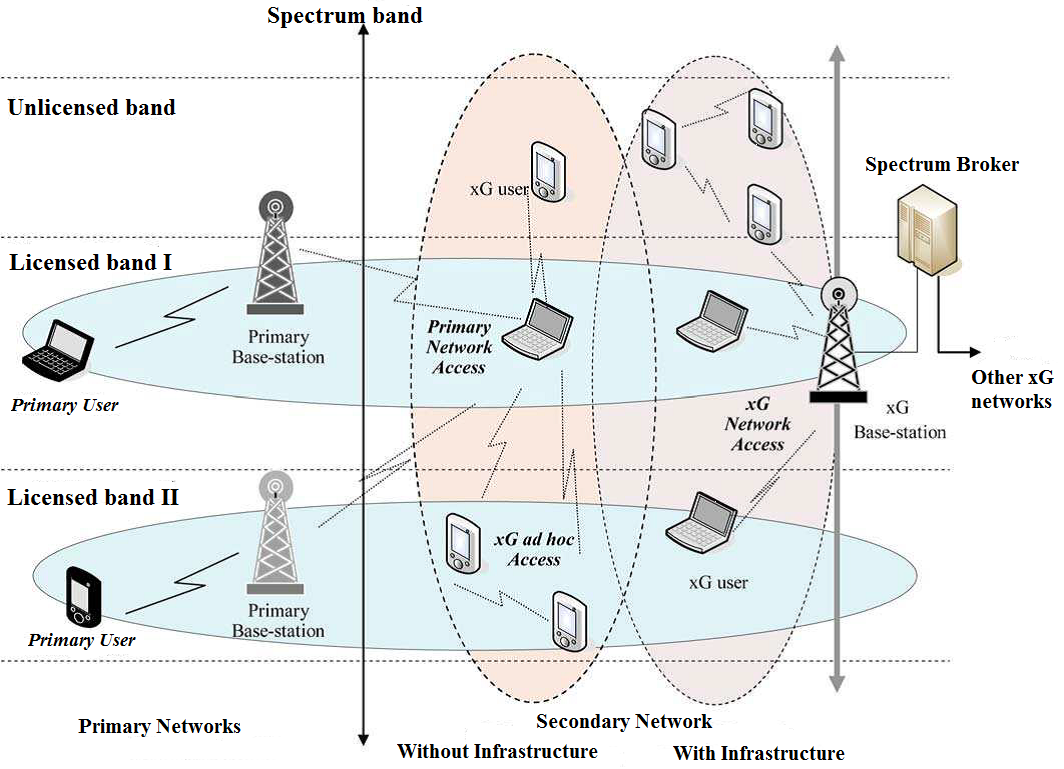
\includegraphics[scale=0.6]{figures/Cognitive-radio-system.png}
	\caption{CRN architecture (source: \cite{r63})}
	\label{CRNsys}
\end{center}
\vspace{-5mm}
\end{figure}



\begin{center}
%\vspace{-2mm}
\begin{figure}[!thb]

\begin{tabular}{cc}
	%	\hspace{30mm}
        \subfigure[The PU is not in transmission (i.e., idle)]{%
            \label{fig:first}
            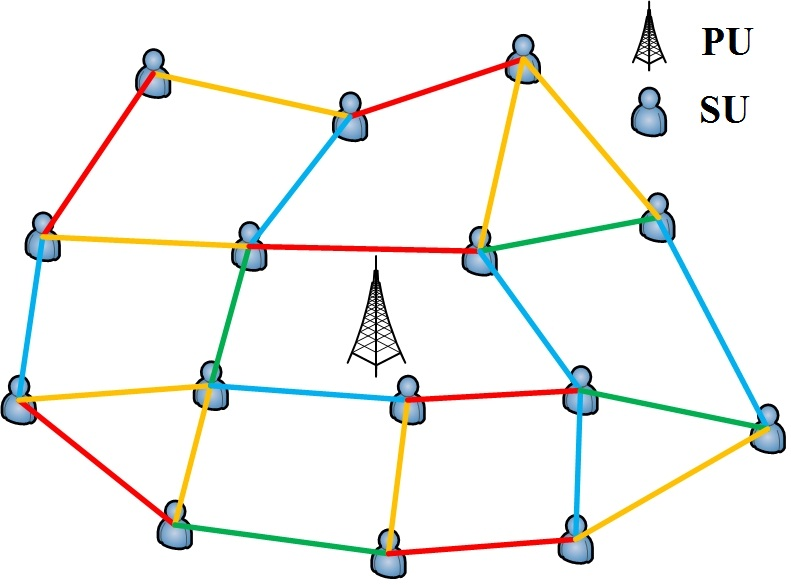
\includegraphics [width=.45\textwidth]{figures/dsa1.jpg} 
        }
        
      %  \vspace{5mm}
       %\hspace{30mm}
        \subfigure[The PU is using the \textit{red} portion of the spectrum for transmission]{%
           \label{fig:second}
           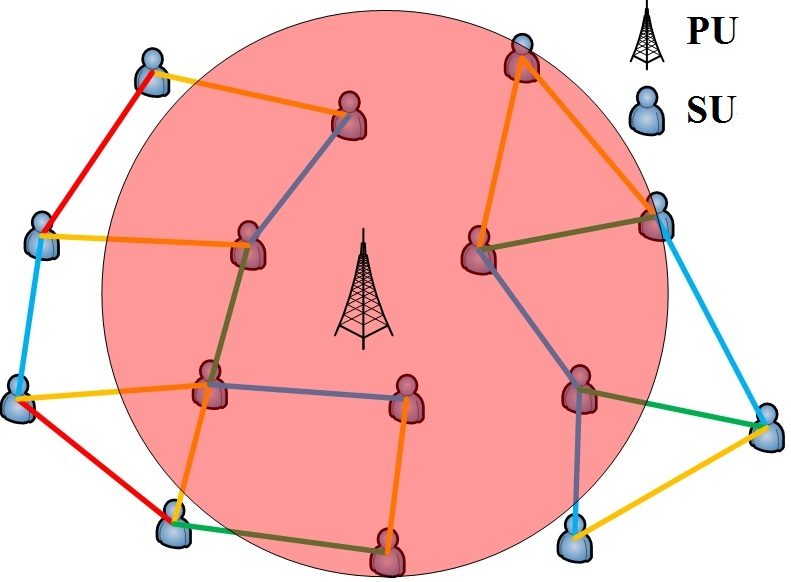
\includegraphics [width=.45\textwidth]{figures/dsa2.jpg}
        }

\end{tabular}
%\vspace{-4mm}
\caption{A CRN scenario with DSA operation. Each coloured line between SUs corresponds to possible connections between them, where different color represents different spectrum fragments. (source: \cite{r64})}%\vspace{-5mm}
\label{DSAop}
\vspace{-10mm}
\end{figure}
\end{center}


